% !TEX program = xelatex
% 智舆 Visual Identity System (VIS) 视觉识别系统手册
\documentclass[12pt,a4paper,fontset=windows]{ctexart}

% ==================== 宏包 ====================
\usepackage{geometry}
\usepackage{graphicx}
\usepackage{xcolor}
\usepackage{tikz}
\usepackage{tcolorbox}
\usepackage{enumitem}
\usepackage{setspace}
\usepackage{titlesec}
\usepackage{array}
\usepackage{float}
\usepackage{fancyhdr}
\usepackage{hyperref}
\usepackage{booktabs}
\usepackage{tabularx}
\usepackage{fontspec}
\usepackage{multicol}
\usepackage{calc}
\usepackage{eso-pic}
\usepackage{transparent}
\usepackage{pdfpages}
\usepackage{tocloft}

\usetikzlibrary{calc,positioning,shadows,patterns,decorations.markings,arrows.meta,shapes.geometric,fit,backgrounds}
\tcbuselibrary{skins,breakable}

% ==================== 页面设置 ====================
\geometry{left=2cm,right=2cm,top=2.5cm,bottom=2cm,headheight=14pt}

% ==================== 品牌色彩定义 ====================
% 主色调
\definecolor{CyberCyan}{HTML}{06B6D4}
\definecolor{CyberCyanLight}{HTML}{22D3EE}
\definecolor{CyberCyanDark}{HTML}{0891B2}
% 强调色
\definecolor{NeonPurple}{HTML}{A855F7}
\definecolor{NeonFuchsia}{HTML}{D946EF}
\definecolor{FuchsiaLight}{HTML}{E879F9}
% 功能色
\definecolor{AlertRed}{HTML}{EF4444}
\definecolor{SuccessGreen}{HTML}{10B981}
\definecolor{WarningAmber}{HTML}{F59E0B}
% 背景色
\definecolor{DeepBlue}{HTML}{0F172A}
\definecolor{DeeperBlue}{HTML}{020617}
\definecolor{SlateGray}{HTML}{334155}
% 中性色
\definecolor{TextPrimary}{HTML}{F8FAFC}
\definecolor{TextSecondary}{HTML}{94A3B8}
\definecolor{GlassBorder}{HTML}{1E293B}
% 辅助
\definecolor{PageBg}{HTML}{FAFBFC}
\definecolor{LightGray}{HTML}{F1F5F9}
\definecolor{MidGray}{HTML}{CBD5E1}

% ==================== 字号 ====================
\newcommand{\chuhao}{\fontsize{42pt}{50pt}\selectfont}
\newcommand{\xiaochu}{\fontsize{36pt}{44pt}\selectfont}
\newcommand{\erhao}{\fontsize{22pt}{28pt}\selectfont}
\newcommand{\xiaoer}{\fontsize{18pt}{24pt}\selectfont}
\newcommand{\sanhao}{\fontsize{16pt}{20pt}\selectfont}
\newcommand{\xiaosan}{\fontsize{15pt}{20pt}\selectfont}
\newcommand{\sihao}{\fontsize{14pt}{18pt}\selectfont}
\newcommand{\xiaosi}{\fontsize{12pt}{16pt}\selectfont}
\newcommand{\wuhao}{\fontsize{10.5pt}{14pt}\selectfont}

% ==================== 超链接 ====================
\hypersetup{
  colorlinks=true,
  linkcolor=CyberCyan,
  urlcolor=CyberCyanDark,
  pdfborder={0 0 0}
}

% ==================== 标题格式 ====================
\titleformat{\section}{\heiti\erhao\color{DeepBlue}}{}{0em}{}[\vspace{2pt}\textcolor{CyberCyan}{\rule{\textwidth}{2pt}}]
\titleformat{\subsection}{\heiti\sanhao\color{DeepBlue}}{\textcolor{CyberCyan}{\thesubsection}}{0.8em}{}
\titleformat{\subsubsection}{\heiti\sihao\color{SlateGray}}{\textcolor{NeonPurple}{\thesubsubsection}}{0.6em}{}
\titlespacing*{\section}{0pt}{24pt}{12pt}
\titlespacing*{\subsection}{0pt}{16pt}{8pt}
\titlespacing*{\subsubsection}{0pt}{12pt}{6pt}

% ==================== 页眉页脚 ====================
\pagestyle{fancy}
\fancyhf{}
\renewcommand{\headrulewidth}{0pt}
\fancyhead[L]{\small\color{TextSecondary}\textbf{智舆} \textbar\ Visual Identity System}
\fancyhead[R]{\small\color{TextSecondary}\thepage}
\fancyfoot[C]{\footnotesize\color{MidGray}\textcopyright\ 2025 智舆 ZhiYu \textbar\ Confidential}

% ==================== 自定义 tcolorbox ====================
% 规范说明框
\newtcolorbox{specbox}[1][]{
  enhanced,
  colback=LightGray,
  colframe=CyberCyan,
  boxrule=0.5pt,
  left=10pt, right=10pt, top=8pt, bottom=8pt,
  arc=1pt,
  fonttitle=\heiti\sihao\color{DeepBlue},
  title={#1},
  coltitle=DeepBlue,
  attach boxed title to top left={xshift=12pt,yshift=-8pt},
  boxed title style={colback=white,colframe=CyberCyan,boxrule=0.5pt,arc=1pt}
}

% 禁止事项框
\newtcolorbox{forbidbox}{
  enhanced,
  colback=AlertRed!5,
  colframe=AlertRed,
  boxrule=0.5pt,
  left=10pt, right=10pt, top=8pt, bottom=8pt,
  arc=1pt,
  fontupper=\xiaosi
}

% 编号标签
\newcommand{\visid}[1]{%
  \tikz[baseline=(char.base)]{
    \node[fill=CyberCyan,text=white,rounded corners=2pt,inner sep=3pt,font=\footnotesize\bfseries\ttfamily] (char) {#1};
  }%
}

% ==================== 目录样式 ====================
\renewcommand{\cfttoctitlefont}{\heiti\erhao\color{DeepBlue}}
\renewcommand{\cftaftertoctitle}{\par\vspace{4pt}\textcolor{CyberCyan}{\rule{\textwidth}{2pt}}}
\renewcommand{\cftsecfont}{\heiti\sihao}
\renewcommand{\cftsubsecfont}{\songti\xiaosi}
\renewcommand{\cftsecleader}{\cftdotfill{\cftdotsep}}

% ==================== 行间距 ====================
\setstretch{1.4}

% ==================== 正文字体 ====================
\AtBeginDocument{\songti\xiaosi}

\begin{document}

% 封面
% ==================== 封面页 ====================
\begin{titlepage}
\newgeometry{left=0cm,right=0cm,top=0cm,bottom=0cm}

\begin{tikzpicture}[remember picture,overlay]
  % 白色背景
  \fill[white] (current page.south west) rectangle (current page.north east);
  
  % 浅灰装饰网格
  \foreach \x in {0,1,...,20} {
    \draw[MidGray,opacity=0.08,line width=0.2pt] (\x,0) -- (\x,29.7);
  }
  \foreach \y in {0,1,...,29} {
    \draw[MidGray,opacity=0.08,line width=0.2pt] (0,\y) -- (21,\y);
  }
  
  % 左侧青色装饰条
  \fill[CyberCyan] (0,0) rectangle (0.35,29.7);
  \fill[CyberCyan,opacity=0.15] (0.35,0) rectangle (0.55,29.7);
  
  % 顶部浅色渐变
  \shade[top color=CyberCyan!8,bottom color=white,opacity=0.8] 
    (0,24) rectangle (21,29.7);
  
  % 底部浅色渐变
  \shade[bottom color=LightGray,top color=white,opacity=0.5] 
    (0,0) rectangle (21,5);
  
  % 装饰圆环
  \draw[CyberCyan,opacity=0.08,line width=1pt] (16,24) circle (3cm);
  \draw[NeonPurple,opacity=0.05,line width=0.5pt] (16,24) circle (3.5cm);
  \draw[CyberCyan,opacity=0.05,line width=0.5pt] (5,4) circle (2cm);
  
  % 装饰六边形
  \node[regular polygon, regular polygon sides=6, minimum size=2.5cm, 
        draw=CyberCyan, opacity=0.06, line width=1pt, rotate=30] at (18,8) {};
  \node[regular polygon, regular polygon sides=6, minimum size=1.5cm, 
        draw=NeonPurple, opacity=0.05, line width=0.5pt, rotate=0] at (3,22) {};

  % ---- 内容区域 ----
  
  % 顶部标签
  \node[anchor=north west,font=\fontsize{9pt}{11pt}\selectfont\ttfamily,text=TextSecondary] 
    at (2,28.5) {VISUAL IDENTITY SYSTEM \textbar\ v1.0 \textbar\ 2025};
  
  % 分隔线
  \draw[CyberCyan,line width=0.5pt] (2,27.8) -- (12,27.8);
  
  % Logo
  \node[anchor=west] at (2,23) {%
    
\includegraphics[height=4.5cm]{picture/logo.png}%
  };
  
  % 品牌名称
  \node[anchor=west,font=\heiti\fontsize{48pt}{56pt}\selectfont,text=DeepBlue] 
    at (2,18) {智舆};
  
  % 英文名
  \node[anchor=west,font=\fontsize{20pt}{24pt}\selectfont\ttfamily,text=CyberCyan] 
    at (2.2,16.2) {ZhiYu};
  
  % 副标题
  \node[anchor=west,font=\heiti\fontsize{13pt}{17pt}\selectfont,text=SlateGray] 
    at (2,14.5) {AI城市舆情态势监测感知与决策推演系统};
  
  % 主标题：VIS
  \draw[CyberCyan,line width=1pt] (2,13) -- (19,13);
  
  \node[anchor=west,font=\fontsize{32pt}{38pt}\selectfont\bfseries,text=DeepBlue] 
    at (2,11) {Visual Identity System};
  
  \node[anchor=west,font=\heiti\fontsize{18pt}{24pt}\selectfont,text=SlateGray] 
    at (2,9.2) {视觉识别系统规范手册};
  
  % 底部信息
  \draw[CyberCyan,line width=0.5pt,opacity=0.4] (2,4.5) -- (19,4.5);
  
  \node[anchor=west,font=\songti\fontsize{10pt}{14pt}\selectfont,text=SlateGray] 
    at (2,3.5) {信阳学院 \textbar\ 首届"数智讯飞杯"AI+创新应用大赛};
  
  \node[anchor=west,font=\ttfamily\fontsize{9pt}{12pt}\selectfont,text=MidGray] 
    at (2,2.5) {CONFIDENTIAL \textbar\ FOR INTERNAL USE ONLY};
  
  % 底部装饰点阵
  \foreach \x in {0,0.3,...,3} {
    \foreach \y in {0,0.3,...,0.9} {
      \fill[CyberCyan,opacity=0.1] (16+\x,1.2+\y) circle (1pt);
    }
  }

\end{tikzpicture}

\restoregeometry
\end{titlepage}
\thispagestyle{empty}


% 目录
\newpage
\tableofcontents
\newpage

% A 基础识别系统
% ==================== A 基础识别系统 ====================

\section{品牌概述}

\subsection{品牌定位}

\textbf{智舆（ZhiYu）}是一款面向城市治理的AI智慧舆情态势监测感知与决策推演系统。品牌视觉以\textbf{赛博朋克（Cyberpunk）}美学为基底，融合\textbf{毛玻璃拟态（Glassmorphism）}与\textbf{数据可视化（Data Visualization）}设计语言，构建"沉浸式、高科技、可信赖"的品牌形象。

\begin{specbox}[品牌核心价值]
\centering
\vspace{4pt}
{\heiti\sanhao\color{CyberCyan} 看得见\quad\textcolor{NeonPurple}{\textbullet}\quad 读得懂\quad\textcolor{NeonPurple}{\textbullet}\quad 判得准\quad\textcolor{NeonPurple}{\textbullet}\quad 做得好}
\vspace{4pt}
\end{specbox}

\subsection{视觉关键词}

\begin{center}
\begin{tikzpicture}
  \foreach \word/\x in {沉浸式/0, 半透明/3.2, 霓虹光效/6.4, 全息投影/9.6, 流动感/12.8} {
    \node[fill=CyberCyan!10,text=CyberCyanDark,rounded corners=1pt,
          inner sep=8pt,font=\heiti\xiaosi,draw=CyberCyan,line width=0.3pt] at (\x,0) {\word};
  }
\end{tikzpicture}
\end{center}

\subsection{品牌架构}

\begin{center}
\begin{tikzpicture}[
  block/.style={rectangle,rounded corners=1pt,draw=CyberCyan,line width=0.8pt,
                fill=CyberCyan!8,text=DeepBlue,minimum width=3.8cm,minimum height=1.2cm,
                font=\heiti\xiaosi,align=center},
  subblock/.style={rectangle,rounded corners=1pt,draw=MidGray,line width=0.5pt,
                   fill=LightGray,text=DeepBlue,minimum width=2.6cm,minimum height=0.9cm,
                   font=\songti\wuhao,align=center},
  arr/.style={-{Stealth[length=5pt]},CyberCyan,line width=0.8pt}
]
  % 顶层
  \node[block,fill=CyberCyan,text=white,line width=1pt] (brand) at (0,0) {智舆 ZhiYu\\品牌标识};
  
  % 二级
  \node[block] (basic) at (-5,-2.5) {A 基础识别\\系统};
  \node[block] (app) at (0,-2.5) {B 应用识别\\系统};
  \node[block] (rule) at (5,-2.5) {C 品牌应用\\规范};
  
  % 三级 - 基础
  \node[subblock] (b1) at (-7,-4.5) {标志规范};
  \node[subblock] (b2) at (-5,-4.5) {色彩系统};
  \node[subblock] (b3) at (-3,-4.5) {字体系统};
  
  % 三级 - 应用
  \node[subblock] (a1) at (-1,-4.5) {界面规范};
  \node[subblock] (a2) at (1,-4.5) {组件设计};
  
  % 三级 - 规范
  \node[subblock] (r1) at (3.5,-4.5) {布局系统};
  \node[subblock] (r2) at (5.5,-4.5) {动效交互};
  \node[subblock] (r3) at (7.5,-4.5) {输出规范};
  
  % 连线
  \draw[arr] (brand) -- (basic);
  \draw[arr] (brand) -- (app);
  \draw[arr] (brand) -- (rule);
  \draw[arr] (basic) -- (b1);
  \draw[arr] (basic) -- (b2);
  \draw[arr] (basic) -- (b3);
  \draw[arr] (app) -- (a1);
  \draw[arr] (app) -- (a2);
  \draw[arr] (rule) -- (r1);
  \draw[arr] (rule) -- (r2);
  \draw[arr] (rule) -- (r3);
\end{tikzpicture}
\end{center}

% ===========================================================
\newpage
\section{标志规范}

\subsection{标志释义}

\visid{A-01} "智舆"Logo以\textbf{立体六边形}为主体框架，顶部延伸\textbf{城市天际线剪影}，中心负空间形成\textbf{对话气泡}，环绕\textbf{莫比乌斯环式数据丝带}。

\begin{figure}[H]
\centering

\includegraphics[width=0.35\textwidth]{picture/logo.png}
\caption{智舆系统标志（标准版）}
\end{figure}

\begin{center}
\renewcommand{\arraystretch}{1.6}
\begin{tabularx}{\textwidth}{>{\centering\arraybackslash\heiti}p{3.5cm} X}
\toprule
\textbf{图形元素} & \textbf{设计寓意} \\
\midrule
六边形框架 & 稳定、高效、互联，象征蜂巢结构的模块化协同能力 \\
城市天际线 & 直观表达"AI+城市"应用场景，呼应3D城市地图核心功能 \\
负空间对话气泡 & 象征舆情核心——公众声音与社会交流，隐喻自然语言交互能力 \\
流动数据丝带 & 代表AI大模型对海量数据的深度分析与逻辑推演 \\
莫比乌斯环 & 象征24小时不间断实时监测与持续迭代优化 \\
\bottomrule
\end{tabularx}
\end{center}

\subsection{标志网格制图}

\visid{A-02} 标志依据标准化网格系统绘制，确保在任何尺寸下的精确还原。网格基准单位 \textbf{a} 等于六边形外接圆直径的 \textbf{1/8}。

\begin{center}
\begin{tikzpicture}
  % 网格
  \foreach \x in {-4,-3.5,...,4} {
    \draw[MidGray,opacity=0.2,line width=0.15pt] (\x,-3.5) -- (\x,3.5);
  }
  \foreach \y in {-3.5,-3,...,3.5} {
    \draw[MidGray,opacity=0.2,line width=0.15pt] (-4,\y) -- (4,\y);
  }
  
  % 主网格（粗线）
  \foreach \x in {-4,-2,0,2,4} {
    \draw[CyberCyan,opacity=0.15,line width=0.3pt] (\x,-3.5) -- (\x,3.5);
  }
  \foreach \y in {-3.5,-1.5,0.5,2.5} {
    \draw[CyberCyan,opacity=0.15,line width=0.3pt] (-4,\y) -- (4,\y);
  }
  
  % Logo（居中）
  \node at (0,0) {
\includegraphics[height=5cm]{picture/logo.png}};
  
  % 中心十字辅助线
  \draw[AlertRed,opacity=0.3,line width=0.3pt,dashed] (0,-3.5) -- (0,3.5);
  \draw[AlertRed,opacity=0.3,line width=0.3pt,dashed] (-4,0) -- (4,0);
  
  % 外接矩形
  \draw[CyberCyan,line width=0.6pt,dashed] (-2.5,-2.8) rectangle (2.5,2.8);
  
  % 标注：基准单位 a
  \draw[{Stealth}-{Stealth},DeepBlue,line width=0.5pt] (-2.5,3.2) -- (-2,3.2);
  \node[above,font=\ttfamily\scriptsize,DeepBlue] at (-2.25,3.2) {a};
  
  % 说明文字区
  \node[anchor=north west,font=\songti\scriptsize,text=SlateGray,text width=5cm] at (5,3) {%
    \textbf{网格参数}\\[4pt]
    基准单位：a = D/8\\
    D = 六边形外接圆直径\\[4pt]
    整体宽高比：约 1:1.12\\
    城市天际线高度：2a\\
    丝带厚度：0.5a\\
    六边形内角：120\textdegree\\[4pt]
    \textcolor{CyberCyan}{---} 定位网格\\
    \textcolor{AlertRed}{- - -} 中轴线\\
    \textcolor{CyberCyan!60}{[~]} 外接边界
  };
\end{tikzpicture}
\end{center}

\begin{specbox}[网格制图使用说明]
\begin{itemize}[leftmargin=1.5em,itemsep=2pt]
  \item 网格制图用于标志的精确复制与大幅面输出校准
  \item 所有曲线控制点须对齐至最近的 0.5a 网格交叉点
  \item 数字化输出时，优先使用矢量格式（SVG/AI），确保无损缩放
  \item 印刷输出时，须以网格制图校验标志比例是否失真
\end{itemize}
\end{specbox}

\subsection{标志安全空间}

\visid{A-03} 标志周围须保留最小安全空间，确保在任何场景下的视觉独立性。安全空间以标志中六边形高度的 \textbf{1/4} 为基准单位 \textbf{X}。

\begin{center}
\begin{tikzpicture}
  % 安全空间示意
  \draw[dashed,CyberCyan,line width=0.5pt] (-3,-2.5) rectangle (3,2.5);
  \draw[dashed,AlertRed,line width=0.3pt] (-2.2,-1.7) rectangle (2.2,1.7);
  \node at (0,0) {
\includegraphics[height=2.8cm]{picture/logo.png}};
  
  % 标注
  \draw[{Stealth}-{Stealth},CyberCyan,line width=0.5pt] (-3,2.7) -- (-2.2,2.7);
  \node[above,font=\ttfamily\scriptsize,CyberCyan] at (-2.6,2.7) {X};
  \draw[{Stealth}-{Stealth},CyberCyan,line width=0.5pt] (3.2,-2.5) -- (3.2,-1.7);
  \node[right,font=\ttfamily\scriptsize,CyberCyan] at (3.2,-2.1) {X};
\end{tikzpicture}
\end{center}

\subsection{标志最小尺寸}

\visid{A-04} 为确保标志清晰可辨，规定以下最小使用尺寸：

\begin{center}
\renewcommand{\arraystretch}{1.5}
\begin{tabular}{lll}
\toprule
\textbf{应用场景} & \textbf{最小宽度} & \textbf{说明} \\
\midrule
印刷媒介 & 20mm & 名片、信封、文档页眉 \\
屏幕显示 & 48px & 网页Favicon、移动端图标 \\
大幅面 & 无上限 & 展板、户外广告 \\
\bottomrule
\end{tabular}
\end{center}

\subsection{标志使用规范}

\visid{A-05} 标志的标准使用场景与禁止操作：

\begin{forbidbox}
\textbf{\color{AlertRed}禁止操作：}
\begin{itemize}[leftmargin=1.5em,itemsep=2pt]
  \item 禁止改变标志比例（拉伸、压缩）
  \item 禁止旋转标志（除设计规范明确允许的角度）
  \item 禁止更改标志配色（须使用标准色或反白版）
  \item 禁止在标志上叠加文字或其他图形元素
  \item 禁止将标志置于杂乱背景上导致辨识度下降
  \item 禁止使用低分辨率标志素材（最低 300dpi 印刷 / 72dpi 屏幕）
\end{itemize}
\end{forbidbox}

\subsection{标志与文字组合规范}

\visid{A-06} 标志与品牌名称的标准组合形式，确保品牌表达的一致性。

\begin{center}
\begin{tikzpicture}
  % 横向组合
  \node[font=\heiti\wuhao,text=SlateGray,anchor=south] at (3.5,4.5) {横向组合（首选）};
  \fill[LightGray,rounded corners=1pt] (0,0.5) rectangle (7,4.3);
  \node[anchor=west] at (0.5,2.4) {
\includegraphics[height=2cm]{picture/logo.png}};
  \node[anchor=west,text=DeepBlue,font=\heiti\fontsize{22pt}{26pt}\selectfont] at (3.2,2.9) {智舆};
  \node[anchor=west,text=CyberCyanDark,font=\ttfamily\fontsize{10pt}{12pt}\selectfont] at (3.2,1.8) {ZhiYu};
  
  % 纵向组合
  \node[font=\heiti\wuhao,text=SlateGray,anchor=south] at (11.5,4.5) {纵向组合};
  \fill[LightGray,rounded corners=1pt] (8.5,0.5) rectangle (14.5,4.3);
  \node at (11.5,3) {
\includegraphics[height=1.5cm]{picture/logo.png}};
  \node[text=DeepBlue,font=\heiti\sihao] at (11.5,1.5) {智舆};
  \node[text=CyberCyanDark,font=\ttfamily\wuhao] at (11.5,0.9) {ZhiYu};
\end{tikzpicture}
\end{center}

\begin{specbox}[组合规范要求]
\begin{itemize}[leftmargin=1.5em,itemsep=2pt]
  \item 标志与文字间距不得小于标志宽度的 \textbf{15\%}
  \item 中文品牌名使用\textbf{黑体}，英文品牌名使用 \textbf{Orbitron} 或等宽字体
  \item 横向组合为首选方案，空间不足时使用纵向组合
  \item 禁止更改标志与文字的相对位置或比例
\end{itemize}
\end{specbox}

\subsection{标志色彩应用版本}

\visid{A-07} 标志在不同背景下的标准色彩应用方案。

\begin{center}
\begin{tikzpicture}
  % 标准版（深色背景）
  \fill[DeepBlue,rounded corners=1pt] (0,0) rectangle (4.5,4);
  \node at (2.25,2.3) {
\includegraphics[height=2cm]{picture/logo.png}};
  \node[text=white,font=\heiti\scriptsize] at (2.25,0.6) {标准版};
  \node[text=TextSecondary,font=\tiny] at (2.25,0.2) {深色背景};
  
  % 反白版（浅色背景）
  \fill[white,rounded corners=1pt,draw=MidGray,line width=0.5pt] (5,0) rectangle (9.5,4);
  \node at (7.25,2.3) {
\includegraphics[height=2cm]{picture/logo.png}};
  \node[text=DeepBlue,font=\heiti\scriptsize] at (7.25,0.6) {浅色背景版};
  \node[text=SlateGray,font=\tiny] at (7.25,0.2) {白色/浅灰背景};
  
  % 单色版
  \fill[LightGray,rounded corners=1pt,draw=MidGray,line width=0.3pt] (10,0) rectangle (14.5,4);
  \node[opacity=0.6] at (12.25,2.3) {
\includegraphics[height=2cm]{picture/logo.png}};
  \node[text=DeepBlue,font=\heiti\scriptsize] at (12.25,0.6) {单色灰度版};
  \node[text=SlateGray,font=\tiny] at (12.25,0.2) {印刷受限场景};
\end{tikzpicture}
\end{center}

\subsection{标志墨稿与反白稿}

\visid{A-08} 标志在特殊印刷条件下的黑白版本规范。

\begin{center}
\begin{tikzpicture}
  % 墨稿（纯黑版）
  \node[font=\heiti\wuhao,text=SlateGray,anchor=south] at (2.25,4.3) {墨稿（纯黑版）};
  \fill[white,rounded corners=1pt,draw=MidGray,line width=0.5pt] (0,0) rectangle (4.5,4);
  \node[opacity=0.15] at (2.25,2.3) {
\includegraphics[height=2cm]{picture/logo.png}};
  \draw[DeepBlue,line width=0.6pt,dashed] (0.8,0.8) rectangle (3.7,3.5);
  \node[text=DeepBlue,font=\ttfamily\tiny] at (2.25,0.4) {K: 100\%};

  % 反白稿
  \node[font=\heiti\wuhao,text=SlateGray,anchor=south] at (7.25,4.3) {反白稿};
  \fill[DeepBlue,rounded corners=1pt] (5,0) rectangle (9.5,4);
  \node at (7.25,2.3) {
\includegraphics[height=2cm]{picture/logo.png}};
  \node[text=TextSecondary,font=\ttfamily\tiny] at (7.25,0.4) {K: 0\% (White)};
  
  % 灰度稿
  \node[font=\heiti\wuhao,text=SlateGray,anchor=south] at (12.25,4.3) {灰度稿};
  \fill[LightGray,rounded corners=1pt,draw=MidGray,line width=0.3pt] (10,0) rectangle (14.5,4);
  \node[opacity=0.5] at (12.25,2.3) {
\includegraphics[height=2cm]{picture/logo.png}};
  \node[text=SlateGray,font=\ttfamily\tiny] at (12.25,0.4) {K: 60\%};
\end{tikzpicture}
\end{center}

\begin{specbox}[墨稿使用场景]
\begin{itemize}[leftmargin=1.5em,itemsep=2pt]
  \item 单色印刷（传真、黑白复印、报纸广告）
  \item 烫金/烫银/压印等特殊工艺
  \item 刻章、钢印、水印等物理载体
\end{itemize}
\end{specbox}

\subsection{标志与Slogan组合}

\visid{A-09} 标志与品牌口号的标准组合形式。

\begin{center}
\begin{tikzpicture}
  % 组合形式1：Logo + Slogan 横向
  \fill[LightGray,rounded corners=1pt] (0,0) rectangle (15,3.5);
  \node[anchor=west] at (0.5,1.8) {
\includegraphics[height=2cm]{picture/logo.png}};
  \node[anchor=west,text=DeepBlue,font=\heiti\fontsize{18pt}{22pt}\selectfont] at (3.2,2.2) {智舆};
  \node[anchor=west,text=CyberCyanDark,font=\ttfamily\wuhao] at (3.2,1.4) {ZhiYu};
  \draw[CyberCyan,line width=0.5pt] (6.5,0.8) -- (6.5,2.8);
  \node[anchor=west,text=SlateGray,font=\songti\xiaosi] at (7,1.8) {看得见 \textbullet\ 读得懂 \textbullet\ 判得准 \textbullet\ 做得好};
\end{tikzpicture}
\end{center}

\begin{specbox}[Slogan组合规范]
\begin{itemize}[leftmargin=1.5em,itemsep=2pt]
  \item Slogan 与标志之间以竖线分隔，间距不小于标志宽度的 \textbf{20\%}
  \item Slogan 字体使用\textbf{宋体/思源宋体}，字号不超过品牌名称的 \textbf{50\%}
  \item 仅在品牌推广场景使用，内部办公文档不附带 Slogan
\end{itemize}
\end{specbox}

\subsection{标志使用错误预演}

\visid{A-10} 以下为常见的标志误用形式，须严格避免。

\begin{center}
\begin{tikzpicture}
  % 错误1：拉伸变形
  \fill[AlertRed!5,rounded corners=1pt] (0,0) rectangle (4.5,3.5);
  \draw[AlertRed,line width=0.5pt,rounded corners=1pt] (0,0) rectangle (4.5,3.5);
  \node[xscale=1.5] at (2.25,2) {
\includegraphics[height=1.2cm]{picture/logo.png}};
  \node[text=AlertRed,font=\heiti\scriptsize] at (2.25,0.5) {拉伸变形};
  \draw[AlertRed,line width=1.5pt] (0.3,0.3) -- (4.2,3.2);
  \draw[AlertRed,line width=1.5pt] (4.2,0.3) -- (0.3,3.2);
  
  % 错误2：旋转
  \fill[AlertRed!5,rounded corners=1pt] (5,0) rectangle (9.5,3.5);
  \draw[AlertRed,line width=0.5pt,rounded corners=1pt] (5,0) rectangle (9.5,3.5);
  \node[rotate=25] at (7.25,2) {
\includegraphics[height=1.2cm]{picture/logo.png}};
  \node[text=AlertRed,font=\heiti\scriptsize] at (7.25,0.5) {任意旋转};
  \draw[AlertRed,line width=1.5pt] (5.3,0.3) -- (9.2,3.2);
  \draw[AlertRed,line width=1.5pt] (9.2,0.3) -- (5.3,3.2);
  
  % 错误3：添加描边/阴影
  \fill[AlertRed!5,rounded corners=1pt] (10,0) rectangle (14.5,3.5);
  \draw[AlertRed,line width=0.5pt,rounded corners=1pt] (10,0) rectangle (14.5,3.5);
  \node[opacity=0.5] at (12.25,2) {
\includegraphics[height=1.2cm]{picture/logo.png}};
  \draw[NeonPurple,line width=2pt,opacity=0.3] (11.2,1.2) rectangle (13.3,2.8);
  \node[text=AlertRed,font=\heiti\scriptsize] at (12.25,0.5) {添加描边/阴影};
  \draw[AlertRed,line width=1.5pt] (10.3,0.3) -- (14.2,3.2);
  \draw[AlertRed,line width=1.5pt] (14.2,0.3) -- (10.3,3.2);
\end{tikzpicture}
\end{center}

\vspace{4pt}

\begin{center}
\begin{tikzpicture}
  % 错误4：更改配色
  \fill[AlertRed!5,rounded corners=1pt] (0,0) rectangle (4.5,3.5);
  \draw[AlertRed,line width=0.5pt,rounded corners=1pt] (0,0) rectangle (4.5,3.5);
  \fill[WarningAmber,opacity=0.3,rounded corners=1pt] (0.5,0.8) rectangle (4,3);
  \node at (2.25,2) {
\includegraphics[height=1.2cm]{picture/logo.png}};
  \node[text=AlertRed,font=\heiti\scriptsize] at (2.25,0.5) {更改配色};
  \draw[AlertRed,line width=1.5pt] (0.3,0.3) -- (4.2,3.2);
  \draw[AlertRed,line width=1.5pt] (4.2,0.3) -- (0.3,3.2);
  
  % 错误5：杂乱背景
  \fill[AlertRed!5,rounded corners=1pt] (5,0) rectangle (9.5,3.5);
  \draw[AlertRed,line width=0.5pt,rounded corners=1pt] (5,0) rectangle (9.5,3.5);
  \foreach \i in {5.2,5.6,...,9.3} {
    \foreach \j in {0.8,1.2,...,3.3} {
      \fill[MidGray,opacity=0.3] (\i,\j) circle (2pt);
    }
  }
  \node at (7.25,2) {
\includegraphics[height=1.2cm]{picture/logo.png}};
  \node[text=AlertRed,font=\heiti\scriptsize] at (7.25,0.5) {杂乱背景};
  \draw[AlertRed,line width=1.5pt] (5.3,0.3) -- (9.2,3.2);
  \draw[AlertRed,line width=1.5pt] (9.2,0.3) -- (5.3,3.2);
  
  % 错误6：低分辨率
  \fill[AlertRed!5,rounded corners=1pt] (10,0) rectangle (14.5,3.5);
  \draw[AlertRed,line width=0.5pt,rounded corners=1pt] (10,0) rectangle (14.5,3.5);
  \node[opacity=0.25] at (12.25,2) {
\includegraphics[height=0.6cm]{picture/logo.png}};
  \node[text=AlertRed,font=\heiti\scriptsize] at (12.25,0.5) {低分辨率};
  \draw[AlertRed,line width=1.5pt] (10.3,0.3) -- (14.2,3.2);
  \draw[AlertRed,line width=1.5pt] (14.2,0.3) -- (10.3,3.2);
\end{tikzpicture}
\end{center}

% ===========================================================
\newpage
\section{色彩系统}

\subsection{主色调}

\visid{A-11} 品牌主色\textbf{Cyber Cyan（赛博青）}代表敏锐、创新与AI的活力，是智舆视觉体系的核心色彩。

\begin{center}
\begin{tikzpicture}
  % 主色大色块
  \fill[CyberCyan,rounded corners=1pt] (0,0) rectangle (6,4);
  \node[text=white,font=\heiti\xiaoer] at (3,2.8) {Cyber Cyan};
  \node[text=white,font=\heiti\xiaosi] at (3,2) {赛博青};
  \node[text=white,font=\ttfamily\wuhao,opacity=0.9] at (3,1.2) {\#06B6D4};
  \node[text=white,font=\ttfamily\scriptsize,opacity=0.7] at (3,0.6) {RGB(6, 182, 212) / Cyan-500};
  
  % 色阶
  \fill[CyberCyanDark,rounded corners=1pt] (7,3) rectangle (9,4);
  \node[text=white,font=\ttfamily\scriptsize] at (8,3.5) {\#0891B2};
  \node[text=white,font=\scriptsize,below] at (8,3) {Dark};
  
  \fill[CyberCyan,rounded corners=1pt] (9.3,3) rectangle (11.3,4);
  \node[text=white,font=\ttfamily\scriptsize] at (10.3,3.5) {\#06B6D4};
  \node[text=white,font=\scriptsize,below] at (10.3,3) {Standard};
  
  \fill[CyberCyanLight,rounded corners=1pt] (11.6,3) rectangle (13.6,4);
  \node[text=DeepBlue,font=\ttfamily\scriptsize] at (12.6,3.5) {\#22D3EE};
  \node[text=DeepBlue,font=\scriptsize,below] at (12.6,3) {Light};
  
  % 使用场景
  \node[anchor=west,font=\heiti\xiaosi,text=DeepBlue] at (7,1.8) {使用场景};
  \node[anchor=west,font=\songti\wuhao,text=SlateGray,text width=7cm] at (7,0.8) {
    核心数据高亮 / 选中状态 / 科技线条 / \\
    按钮主色 / 图表主色 / 链接文字
  };
\end{tikzpicture}
\end{center}

\subsection{强调色}

\visid{A-12} 强调色用于丰富视觉层次，与主色形成互补关系。

\begin{center}
\begin{tikzpicture}
  % Neon Purple
  \fill[NeonPurple,rounded corners=1pt] (0,0) rectangle (4.2,3);
  \node[text=white,font=\heiti\sihao] at (2.1,2.2) {Neon Purple};
  \node[text=white,font=\heiti\wuhao] at (2.1,1.5) {霓虹紫};
  \node[text=white,font=\ttfamily\scriptsize] at (2.1,0.8) {\#A855F7 / Purple-500};
  \node[text=white,font=\scriptsize,opacity=0.8] at (2.1,0.3) {辅助图形 / 渐变光晕};
  
  % Neon Fuchsia
  \fill[NeonFuchsia,rounded corners=1pt] (4.6,0) rectangle (8.8,3);
  \node[text=white,font=\heiti\sihao] at (6.7,2.2) {Neon Fuchsia};
  \node[text=white,font=\heiti\wuhao] at (6.7,1.5) {霓虹品红};
  \node[text=white,font=\ttfamily\scriptsize] at (6.7,0.8) {\#D946EF / Fuchsia-500};
  \node[text=white,font=\scriptsize,opacity=0.8] at (6.7,0.3) {次要强调 / 悬停高亮};
  
  % Alert Red
  \fill[AlertRed,rounded corners=1pt] (9.2,0) rectangle (13.4,3);
  \node[text=white,font=\heiti\sihao] at (11.3,2.2) {Alert Red};
  \node[text=white,font=\heiti\wuhao] at (11.3,1.5) {警报红};
  \node[text=white,font=\ttfamily\scriptsize] at (11.3,0.8) {\#EF4444 / Red-500};
  \node[text=white,font=\scriptsize,opacity=0.8] at (11.3,0.3) {警报 / 异常 / 删除};
\end{tikzpicture}
\end{center}

\subsection{功能色}

\visid{A-13} 功能色用于传达系统状态信息，具有明确的语义。

\begin{center}
\begin{tikzpicture}
  % Success
  \fill[SuccessGreen,rounded corners=1pt] (0,0) rectangle (3.6,2.2);
  \node[text=white,font=\heiti\xiaosi] at (1.8,1.5) {Success Green};
  \node[text=white,font=\ttfamily\scriptsize] at (1.8,0.8) {\#10B981};
  \node[text=white,font=\scriptsize,opacity=0.8] at (1.8,0.3) {成功 / 正常 / 正面};
  
  % Warning
  \fill[WarningAmber,rounded corners=1pt] (4,0) rectangle (7.6,2.2);
  \node[text=white,font=\heiti\xiaosi] at (5.8,1.5) {Warning Amber};
  \node[text=white,font=\ttfamily\scriptsize] at (5.8,0.8) {\#F59E0B};
  \node[text=white,font=\scriptsize,opacity=0.8] at (5.8,0.3) {警告 / 待处理};
  
  % Alert
  \fill[AlertRed,rounded corners=1pt] (8,0) rectangle (11.6,2.2);
  \node[text=white,font=\heiti\xiaosi] at (9.8,1.5) {Alert Red};
  \node[text=white,font=\ttfamily\scriptsize] at (9.8,0.8) {\#EF4444};
  \node[text=white,font=\scriptsize,opacity=0.8] at (9.8,0.3) {危险 / 错误 / 负面};
\end{tikzpicture}
\end{center}

\subsection{背景与中性色}

\visid{A-14} 背景色系采用深色模式（Dark Mode）为基底，突显光效与数据图表。

\begin{center}
\begin{tikzpicture}
  % 深色背景序列
  \fill[DeeperBlue,rounded corners=1pt] (0,0) rectangle (2.8,2.8);
  \node[text=white,font=\heiti\scriptsize] at (1.4,2) {Deeper Blue};
  \node[text=TextSecondary,font=\ttfamily\tiny] at (1.4,1.4) {\#020617};
  \node[text=TextSecondary,font=\tiny] at (1.4,0.8) {Slate-950};
  \node[text=TextSecondary,font=\tiny] at (1.4,0.3) {最深背景};
  
  \fill[DeepBlue,rounded corners=1pt] (3.1,0) rectangle (5.9,2.8);
  \node[text=white,font=\heiti\scriptsize] at (4.5,2) {Deep Blue};
  \node[text=TextSecondary,font=\ttfamily\tiny] at (4.5,1.4) {\#0F172A};
  \node[text=TextSecondary,font=\tiny] at (4.5,0.8) {Slate-900};
  \node[text=TextSecondary,font=\tiny] at (4.5,0.3) {主背景};
  
  \fill[SlateGray,rounded corners=1pt] (6.2,0) rectangle (9,2.8);
  \node[text=white,font=\heiti\scriptsize] at (7.6,2) {Slate Gray};
  \node[text=TextSecondary,font=\ttfamily\tiny] at (7.6,1.4) {\#334155};
  \node[text=TextSecondary,font=\tiny] at (7.6,0.8) {Slate-700};
  \node[text=TextSecondary,font=\tiny] at (7.6,0.3) {卡片/分割};
  
  % 文字色
  \fill[white,rounded corners=1pt,draw=MidGray,line width=0.3pt] (9.3,0) rectangle (12.1,2.8);
  \node[text=DeepBlue,font=\heiti\scriptsize] at (10.7,2) {Text Primary};
  \node[text=SlateGray,font=\ttfamily\tiny] at (10.7,1.4) {\#F8FAFC};
  \node[text=SlateGray,font=\tiny] at (10.7,0.8) {Slate-50};
  \node[text=SlateGray,font=\tiny] at (10.7,0.3) {主要文字};
  
  \fill[TextSecondary,rounded corners=1pt] (12.4,0) rectangle (15.2,2.8);
  \node[text=white,font=\heiti\scriptsize] at (13.8,2) {Text Secondary};
  \node[text=white,font=\ttfamily\tiny] at (13.8,1.4) {\#94A3B8};
  \node[text=white,font=\tiny] at (13.8,0.8) {Slate-400};
  \node[text=white,font=\tiny] at (13.8,0.3) {次要文字};
\end{tikzpicture}
\end{center}

\subsection{色彩组合规范}

\visid{A-15} 以下为标准色彩搭配方案，确保对比度与可读性。

\begin{center}
\renewcommand{\arraystretch}{1.6}
\begin{tabularx}{\textwidth}{>{\centering\arraybackslash}p{3cm} >{\centering\arraybackslash}p{3cm} >{\centering\arraybackslash}p{3cm} X}
\toprule
\textbf{场景} & \textbf{背景色} & \textbf{前景色} & \textbf{说明} \\
\midrule
深色界面主文字 & \colorbox{DeepBlue}{\textcolor{white}{\footnotesize\#0F172A}} & \colorbox{white}{\footnotesize\#F8FAFC} & WCAG AAA \\
深色界面次要文字 & \colorbox{DeepBlue}{\textcolor{white}{\footnotesize\#0F172A}} & \colorbox{TextSecondary}{\textcolor{white}{\footnotesize\#94A3B8}} & WCAG AA \\
青色高亮文字 & \colorbox{DeepBlue}{\textcolor{white}{\footnotesize\#0F172A}} & \colorbox{CyberCyanLight}{\footnotesize\#22D3EE} & 数据标注 \\
印刷正文 & 白色纸张 & \colorbox{DeepBlue}{\textcolor{white}{\footnotesize\#0F172A}} & 最高对比度 \\
\bottomrule
\end{tabularx}
\end{center}

\begin{forbidbox}
\textbf{\color{AlertRed}色彩禁止操作：}
\begin{itemize}[leftmargin=1.5em,itemsep=2pt]
  \item 禁止在浅色背景上使用 Cyber Cyan 作为正文文字色（对比度不足）
  \item 禁止将 Alert Red 与 Success Green 直接相邻使用
  \item 禁止修改标准色值（色差 $\Delta E < 3$ 方可视为一致）
  \item 禁止在非深色背景上使用霓虹光效（Neon Glow）
\end{itemize}
\end{forbidbox}

\subsection{印刷色值对照表}

\visid{A-16} 印刷输出时须使用 CMYK 色值，确保跨媒介色彩一致性。

\begin{center}
\renewcommand{\arraystretch}{1.6}
\begin{tabularx}{\textwidth}{>{\heiti\centering\arraybackslash}p{2.8cm} >{\centering\arraybackslash}p{2.4cm} >{\centering\arraybackslash}p{2.8cm} >{\centering\arraybackslash}p{2.8cm} X}
\toprule
\textbf{色彩名称} & \textbf{HEX} & \textbf{RGB} & \textbf{CMYK} & \textbf{Pantone (近似)} \\
\midrule
\colorbox{CyberCyan}{\textcolor{white}{\small Cyber Cyan}} & \#06B6D4 & 6, 182, 212 & C78 M0 Y15 K0 & 3125 C \\
\colorbox{CyberCyanLight}{\small Cyan Light} & \#22D3EE & 34, 211, 238 & C65 M0 Y8 K0 & 305 C \\
\colorbox{NeonPurple}{\textcolor{white}{\small Neon Purple}} & \#A855F7 & 168, 85, 247 & C45 M70 Y0 K0 & 2655 C \\
\colorbox{NeonFuchsia}{\textcolor{white}{\small Neon Fuchsia}} & \#D946EF & 217, 70, 239 & C25 M75 Y0 K0 & 253 C \\
\colorbox{AlertRed}{\textcolor{white}{\small Alert Red}} & \#EF4444 & 239, 68, 68 & C0 M82 Y70 K0 & 185 C \\
\colorbox{SuccessGreen}{\textcolor{white}{\small Success Green}} & \#10B981 & 16, 185, 129 & C70 M0 Y50 K0 & 3405 C \\
\colorbox{WarningAmber}{\textcolor{white}{\small Warning Amber}} & \#F59E0B & 245, 158, 11 & C0 M40 Y95 K0 & 137 C \\
\colorbox{DeepBlue}{\textcolor{white}{\small Deep Blue}} & \#0F172A & 15, 23, 42 & C90 M80 Y40 K60 & 5395 C \\
\bottomrule
\end{tabularx}
\end{center}

\begin{specbox}[印刷注意事项]
\begin{itemize}[leftmargin=1.5em,itemsep=2pt]
  \item CMYK 色值在不同印刷设备上可能存在偏差，打样确认后方可批量印刷
  \item 霓虹色系（Cyan / Purple / Fuchsia）在 CMYK 下饱和度会降低，重要物料建议使用专色（Pantone）
  \item 大面积深色印刷建议总墨量控制在 280\% 以内，避免背印透色
\end{itemize}
\end{specbox}

% ===========================================================
\newpage
\section{字体系统}

\subsection{品牌字体}

\visid{A-17} 智舆品牌采用以下字体体系，兼顾科技感与中文可读性。

\begin{center}
\begin{tikzpicture}
  % 主字体卡片
  \fill[LightGray,rounded corners=1pt] (0,0) rectangle (7.5,5.5);
  \draw[CyberCyan,rounded corners=1pt,line width=0.5pt] (0,0) rectangle (7.5,5.5);
  \node[text=CyberCyanDark,font=\heiti\sihao,anchor=north west] at (0.5,5) {主字体 / Primary};
  \draw[CyberCyan,line width=0.5pt] (0.5,4.3) -- (7,4.3);
  \node[text=DeepBlue,font=\fontsize{24pt}{28pt}\selectfont,anchor=west] at (0.5,3.4) {Alibaba PuHuiTi 2.0};
  \node[text=SlateGray,font=\xiaosi,anchor=west] at (0.5,2.3) {阿里巴巴普惠体 2.0};
  \node[text=SlateGray,font=\wuhao,anchor=west,text width=6.5cm] at (0.5,1.3) {
    用途：正文、界面文字、数据标签\\
    特性：免费商用、清晰易读、多字重
  };
  
  % 标题/科技字体
  \fill[LightGray,rounded corners=1pt] (8,0) rectangle (15.5,5.5);
  \draw[CyberCyan,rounded corners=1pt,line width=0.5pt] (8,0) rectangle (15.5,5.5);
  \node[text=CyberCyanDark,font=\heiti\sihao,anchor=north west] at (8.5,5) {科技字体 / Tech};
  \draw[CyberCyan,line width=0.5pt] (8.5,4.3) -- (15,4.3);
  \node[text=DeepBlue,font=\fontsize{24pt}{28pt}\selectfont,anchor=west] at (8.5,3.4) {Orbitron};
  \node[text=SlateGray,font=\xiaosi,anchor=west] at (8.5,2.3) {轨道字体};
  \node[text=SlateGray,font=\wuhao,anchor=west,text width=6.5cm] at (8.5,1.3) {
    用途：标题数字、仪表盘、KPI指标\\
    特性：几何感、未来风、等宽数字
  };
\end{tikzpicture}
\end{center}

\vspace{8pt}

\begin{center}
\begin{tikzpicture}
  % 西文字体
  \fill[LightGray,rounded corners=1pt,draw=MidGray,line width=0.3pt] (0,0) rectangle (7.5,4);
  \node[text=DeepBlue,font=\heiti\sihao,anchor=north west] at (0.5,3.6) {西文正文 / Sans-serif};
  \draw[MidGray,line width=0.3pt] (0.5,2.9) -- (7,2.9);
  \node[text=DeepBlue,font=\fontsize{20pt}{24pt}\selectfont,anchor=west] at (0.5,2) {Inter};
  \node[text=SlateGray,font=\wuhao,anchor=west,text width=6.5cm] at (0.5,0.8) {
    用途：英文正文、按钮文字、导航\\
    备选：Segoe UI / system-ui
  };
  
  % 等宽字体
  \fill[LightGray,rounded corners=1pt,draw=MidGray,line width=0.3pt] (8,0) rectangle (15.5,4);
  \node[text=DeepBlue,font=\heiti\sihao,anchor=north west] at (8.5,3.6) {等宽字体 / Monospace};
  \draw[MidGray,line width=0.3pt] (8.5,2.9) -- (15,2.9);
  \node[text=DeepBlue,font=\fontsize{20pt}{24pt}\selectfont\ttfamily,anchor=west] at (8.5,2) {JetBrains Mono};
  \node[text=SlateGray,font=\wuhao,anchor=west,text width=6.5cm] at (8.5,0.8) {
    用途：代码片段、数据编号、技术标注\\
    备选：Fira Code / Consolas
  };
\end{tikzpicture}
\end{center}

\subsection{字体层级}

\visid{A-18} 字体层级遵循以下规范，确保信息的视觉优先级清晰。

\begin{center}
\renewcommand{\arraystretch}{1.8}
\begin{tabularx}{\textwidth}{>{\centering\arraybackslash}p{2.5cm} >{\centering\arraybackslash}p{2cm} >{\centering\arraybackslash}p{2cm} >{\centering\arraybackslash}p{2cm} X}
\toprule
\textbf{层级} & \textbf{字号} & \textbf{字重} & \textbf{行高} & \textbf{用途} \\
\midrule
H1 大标题 & 32px & Bold & 1.2 & 页面主标题 \\
H2 章标题 & 24px & Bold & 1.3 & 模块标题 \\
H3 节标题 & 18px & SemiBold & 1.4 & 卡片标题 \\
Body 正文 & 14px & Regular & 1.6 & 正文内容 \\
Caption 标注 & 12px & Regular & 1.5 & 辅助说明 \\
Data 数据 & 28--48px & Bold & 1.1 & KPI/仪表盘数字 \\
\bottomrule
\end{tabularx}
\end{center}

\subsection{辅助图形系统}

\visid{A-19} 品牌辅助图形源自Logo中的核心元素，用于丰富视觉层次。

\begin{center}
\begin{tikzpicture}
  % 六边形网格
  \begin{scope}[shift={(0,0)}]
    \node[font=\heiti\xiaosi,text=DeepBlue,anchor=south] at (2,3.5) {六边形网格};
    \foreach \i/\j in {0/0,1.5/0,0.75/1.3,2.25/1.3,0/2.6,1.5/2.6} {
      \node[regular polygon,regular polygon sides=6,minimum size=1.3cm,
            draw=CyberCyan,line width=0.5pt,opacity=0.6,rotate=30] at (\i,\j) {};
    }
  \end{scope}
  
  % 数据流线
  \begin{scope}[shift={(5.5,0)}]
    \node[font=\heiti\xiaosi,text=DeepBlue,anchor=south] at (2,3.5) {数据流线};
    \draw[CyberCyan,line width=1.5pt,opacity=0.8,
          decoration={markings,mark=at position 0.3 with {\arrow{Stealth}},
                      mark=at position 0.7 with {\arrow{Stealth}}},
          postaction={decorate}]
      (0,0.5) .. controls (1,2.5) and (3,1) .. (4,3);
    \draw[NeonPurple,line width=1pt,opacity=0.5]
      (0,1.5) .. controls (1.5,3) and (2.5,0) .. (4,2);
    \draw[CyberCyanLight,line width=0.5pt,opacity=0.3]
      (0.5,0) .. controls (2,2) and (3,1.5) .. (3.5,3.2);
  \end{scope}
  
  % 光晕圆环
  \begin{scope}[shift={(11.5,0)}]
    \node[font=\heiti\xiaosi,text=DeepBlue,anchor=south] at (1.8,3.5) {光晕圆环};
    \draw[CyberCyan,line width=1.5pt,opacity=0.6] (1.8,1.5) circle (1.2cm);
    \draw[NeonPurple,line width=1pt,opacity=0.3] (1.8,1.5) circle (1.5cm);
    \draw[CyberCyanLight,line width=0.5pt,opacity=0.2] (1.8,1.5) circle (1.8cm);
    \fill[CyberCyan,opacity=0.15] (1.8,1.5) circle (0.6cm);
  \end{scope}
\end{tikzpicture}
\end{center}

\begin{specbox}[辅助图形使用原则]
\begin{itemize}[leftmargin=1.5em,itemsep=2pt]
  \item 辅助图形须始终保持\textbf{低透明度}（10\%--30\%），避免喧宾夺主
  \item 深色背景使用青色/紫色光效，印刷场景使用灰度线条版本
  \item 六边形网格可用于文档背景、PPT底纹、名片装饰等
  \item 数据流线可用于分割线、过渡区域、页面装饰
\end{itemize}
\end{specbox}


% B 应用识别系统
% ==================== B 应用识别系统 ====================

\newpage
\section{界面设计规范}

\subsection{设计风格定义}

\visid{B-01} 智舆系统界面采用 \textbf{Cyberpunk + Glassmorphism + Data Vis} 三位一体的设计风格。

\begin{center}
\begin{tikzpicture}
  % 三圆交集示意
  \begin{scope}[opacity=0.15]
    \fill[CyberCyan] (0,0) circle (2.2cm);
    \fill[NeonPurple] (2.5,0) circle (2.2cm);
    \fill[SuccessGreen] (1.25,2) circle (2.2cm);
  \end{scope}
  % 标签
  \node[font=\heiti\sihao,text=CyberCyanDark] at (-0.8,-0.5) {Cyberpunk};
  \node[font=\songti\wuhao,text=SlateGray] at (-0.8,-1.1) {赛博朋克};
  
  \node[font=\heiti\sihao,text=NeonPurple] at (3.3,-0.5) {Glassmorphism};
  \node[font=\songti\wuhao,text=SlateGray] at (3.3,-1.1) {毛玻璃拟态};
  
  \node[font=\heiti\sihao,text=SuccessGreen!80!black] at (1.25,2.8) {Data Vis};
  \node[font=\songti\wuhao,text=SlateGray] at (1.25,2.2) {数据可视化};
  
  % 交集中心
  \node[font=\heiti\xiaosan,text=DeepBlue] at (1.25,0.7) {智舆};
\end{tikzpicture}
\end{center}

\begin{center}
\renewcommand{\arraystretch}{1.6}
\begin{tabularx}{\textwidth}{>{\centering\arraybackslash\heiti}p{3cm} X X}
\toprule
\textbf{风格维度} & \textbf{视觉特征} & \textbf{技术实现} \\
\midrule
Cyberpunk & 深色基底、霓虹发光、扫描线纹理、角落装饰 & CSS box-shadow / text-shadow / linear-gradient \\
Glassmorphism & 半透明卡片、背景模糊、微透光边框 & backdrop-filter: blur / bg-opacity / border-white/10 \\
Data Vis & 动态图表、脉冲标记、实时数据流、热力渲染 & ECharts / Three.js / 高德地图 GLCustomLayer \\
\bottomrule
\end{tabularx}
\end{center}

\subsection{界面布局结构}

\visid{B-02} 系统主界面采用\textbf{仪表盘布局（Dashboard Layout）}，以3D地图为核心视图。

\begin{center}
\begin{tikzpicture}[
  panel/.style={rounded corners=1pt,draw=CyberCyan,line width=0.6pt,fill=DeepBlue,fill opacity=0.9,text opacity=1},
  label/.style={font=\scriptsize\heiti,text=CyberCyanLight}
]
  % 整体框架
  \fill[DeeperBlue,rounded corners=1pt] (-0.3,-0.3) rectangle (15.3,9.3);
  
  % 顶部导航 - Dynamic Island
  \draw[panel] (0,8.2) rectangle (15,9) node[pos=0.5,label] {Header / Dynamic Island -- 时间 | 城市选择 | 功能入口 | 用户};
  
  % 左侧边栏
  \draw[panel] (0,0) rectangle (3.5,8) node[pos=0.5,label,text width=3cm,align=center] {Left Sidebar\\舆情列表\\筛选条件\\统计概览};
  
  % 中央主视图
  \fill[DeepBlue,rounded corners=1pt,opacity=0.5] (3.7,0) rectangle (11,8);
  \draw[CyberCyan,line width=0.6pt,rounded corners=1pt] (3.7,0) rectangle (11,8);
  \node[label,font=\heiti\xiaosi\color{CyberCyanLight}] at (7.35,4) {3D Map View};
  \node[label,font=\songti\scriptsize\color{TextSecondary}] at (7.35,3.2) {高德地图3D + Three.js GLCustomLayer};
  % 装饰：脉冲点
  \fill[CyberCyan,opacity=0.6] (5.5,5.5) circle (3pt);
  \fill[CyberCyan,opacity=0.3] (5.5,5.5) circle (6pt);
  \fill[AlertRed,opacity=0.6] (8.2,6.2) circle (3pt);
  \fill[AlertRed,opacity=0.3] (8.2,6.2) circle (6pt);
  \fill[WarningAmber,opacity=0.6] (9.5,2.8) circle (3pt);
  \fill[WarningAmber,opacity=0.3] (9.5,2.8) circle (6pt);
  
  % 右侧边栏
  \draw[panel] (11.2,4.2) rectangle (15,8) node[pos=0.5,label,text width=3.2cm,align=center] {Right Panel\\舆情详情\\分析报告\\AI助手};
  
  \draw[panel] (11.2,0) rectangle (15,4) node[pos=0.5,label,text width=3.2cm,align=center] {Widgets\\图表面板\\趋势分析\\KPI指标};
  
  % 底部工具栏
  \draw[panel,fill opacity=0.7] (3.7,-0.2) -- (3.7,0) -- (11,0) -- (11,-0.2) -- cycle;
  
  % 层级标注
  \node[anchor=west,font=\tiny\ttfamily,text=NeonPurple] at (0,9.5) {Layer 1: Overlay Panels};
  \node[anchor=west,font=\tiny\ttfamily,text=CyberCyan] at (5,9.5) {Layer 0: 3D Map Background};
\end{tikzpicture}
\end{center}

\subsection{响应式断点}

\visid{B-03} 系统支持多终端自适应布局。

\begin{center}
\renewcommand{\arraystretch}{1.5}
\begin{tabularx}{\textwidth}{>{\centering\arraybackslash\heiti}p{2.5cm} >{\centering\arraybackslash}p{2cm} X}
\toprule
\textbf{断点} & \textbf{宽度} & \textbf{布局策略} \\
\midrule
Desktop XL & $\geq$1440px & 完整三栏布局（侧边栏 + 地图 + 右面板） \\
Desktop LG & $\geq$1024px & 三栏布局，右面板可折叠 \\
Tablet MD & $\geq$768px & 双栏布局，侧边栏收起为图标模式 \\
Mobile SM & $<$768px & 单列布局，地图全屏背景，功能面板底部抽屉唤起 \\
\bottomrule
\end{tabularx}
\end{center}

% ===========================================================
\newpage
\section{核心组件设计}

\subsection{玻璃面板 GlassPanel}

\visid{B-04} 所有信息面板采用统一的毛玻璃效果，确保背景可见并增强空间层次感。

\begin{center}
\begin{tikzpicture}
  % 模拟深色背景
  \fill[DeepBlue,rounded corners=1pt] (-0.5,-0.5) rectangle (15.5,5.5);
  
  % 背景装饰
  \fill[CyberCyan,opacity=0.08] (3,1) circle (2cm);
  \fill[NeonPurple,opacity=0.06] (10,3) circle (1.5cm);
  
  % GlassPanel 示例
  \fill[SlateGray,opacity=0.4,rounded corners=1pt] (1,0.5) rectangle (7,4.5);
  \draw[white,opacity=0.1,rounded corners=1pt,line width=0.5pt] (1,0.5) rectangle (7,4.5);
  
  % 角落装饰
  \draw[CyberCyan,line width=0.8pt] (1,4.5) -- (1,4) (1,4.5) -- (1.5,4.5);
  \draw[CyberCyan,line width=0.8pt] (7,0.5) -- (7,1) (7,0.5) -- (6.5,0.5);
  
  % 扫描线效果提示
  \foreach \y in {0.7,0.9,...,4.3} {
    \draw[white,opacity=0.03,line width=0.3pt] (1.1,\y) -- (6.9,\y);
  }
  
  \node[text=CyberCyanLight,font=\heiti\xiaosi,anchor=north west] at (1.4,4.2) {GlassPanel};
  \node[text=TextSecondary,font=\songti\scriptsize,anchor=north west,text width=5cm] at (1.4,3.5) {
    背景: bg-slate-900/40\\
    模糊: backdrop-blur-xl (12px)\\
    边框: border-white/10\\
    圆角: rounded-2xl (16px)\\
    阴影: shadow-cyan-500/10
  };
  
  % CSS代码示例
  \node[anchor=north west,font=\ttfamily\tiny,text=CyberCyanLight,text width=6.5cm] at (8.5,4.8) {%
    .cyber-card \{\\
    \quad background: rgba(15,23,42,0.6);\\
    \quad backdrop-filter: blur(12px);\\
    \quad border: 1px solid rgba(255,255,255,0.1);\\
    \quad border-radius: 16px;\\
    \quad transition: all 0.3s ease;\\
    \}\\[4pt]
    .cyber-card:hover \{\\
    \quad border-color: rgba(6,182,212,0.5);\\
    \quad box-shadow: 0 0 10px rgba(6,182,212,0.5);\\
    \}
  };
\end{tikzpicture}
\end{center}

\subsection{霓虹按钮 NeonButton}

\visid{B-05} 按钮组件遵循三种语义变体，对应不同操作类型。

\begin{center}
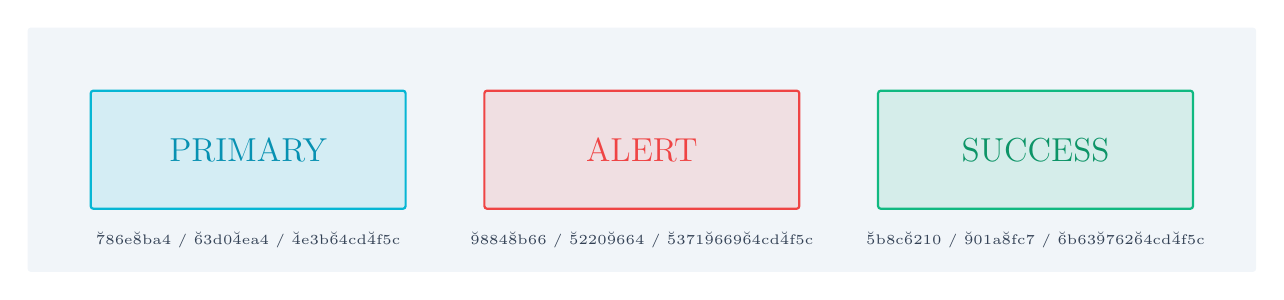
\begin{tikzpicture}
  % \u6d45\u8272\u80cc\u666f
  \fill[LightGray,rounded corners=1pt] (-0.3,-0.3) rectangle (15.3,2.8);
  
  % Primary
  \fill[CyberCyan,opacity=0.12,rounded corners=1pt] (0.5,0.5) rectangle (4.5,2);
  \draw[CyberCyan,rounded corners=1pt,line width=0.8pt] (0.5,0.5) rectangle (4.5,2);
  \node[text=CyberCyanDark,font=\heiti\xiaosi] at (2.5,1.25) {PRIMARY};
  \node[text=SlateGray,font=\tiny] at (2.5,0.1) {\u786e\u8ba4 / \u63d0\u4ea4 / \u4e3b\u64cd\u4f5c};
  
  % Alert
  \fill[AlertRed,opacity=0.12,rounded corners=1pt] (5.5,0.5) rectangle (9.5,2);
  \draw[AlertRed,rounded corners=1pt,line width=0.8pt] (5.5,0.5) rectangle (9.5,2);
  \node[text=AlertRed,font=\heiti\xiaosi] at (7.5,1.25) {ALERT};
  \node[text=SlateGray,font=\tiny] at (7.5,0.1) {\u9884\u8b66 / \u5220\u9664 / \u5371\u9669\u64cd\u4f5c};
  
  % Success
  \fill[SuccessGreen,opacity=0.12,rounded corners=1pt] (10.5,0.5) rectangle (14.5,2);
  \draw[SuccessGreen,rounded corners=1pt,line width=0.8pt] (10.5,0.5) rectangle (14.5,2);
  \node[text=SuccessGreen!80!black,font=\heiti\xiaosi] at (12.5,1.25) {SUCCESS};
  \node[text=SlateGray,font=\tiny] at (12.5,0.1) {\u5b8c\u6210 / \u901a\u8fc7 / \u6b63\u9762\u64cd\u4f5c};
\end{tikzpicture}
\end{center}

\begin{specbox}[按钮交互规范]
\begin{itemize}[leftmargin=1.5em,itemsep=2pt]
  \item \textbf{Hover}: 背景透明度 20\% $\to$ 40\%，增加霓虹光晕 box-shadow
  \item \textbf{Active}: 背景透明度降至 30\%，轻微缩放 scale(0.98)
  \item \textbf{Disabled}: 整体透明度降至 40\%，禁用指针事件
  \item 字体统一使用 \texttt{font-mono uppercase tracking-wider text-sm}
\end{itemize}
\end{specbox}

\subsection{导航栏 Dynamic Island}

\visid{B-06} 顶部导航采用\textbf{灵动岛（Dynamic Island）}风格，整合状态与菜单，节省空间。

\begin{center}
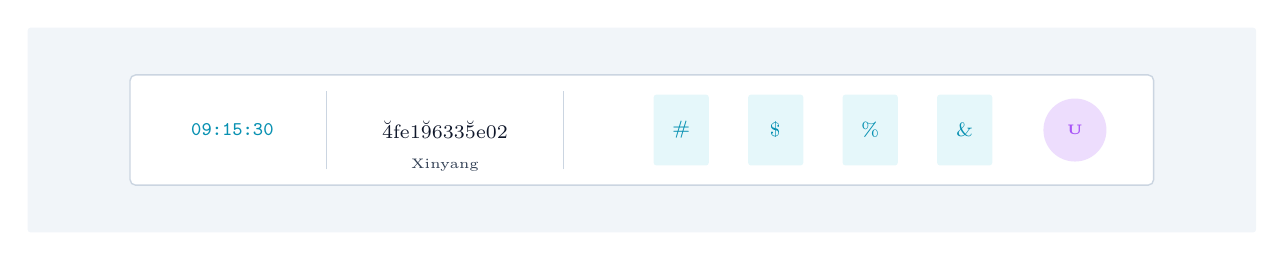
\begin{tikzpicture}
  % \u6d45\u8272\u80cc\u666f
  \fill[LightGray,rounded corners=1pt] (-0.3,-0.3) rectangle (15.3,2.3);
  
  % \u5bfc\u822a\u680f\u4e3b\u4f53
  \fill[white,rounded corners=2pt] (1,0.3) rectangle (14,1.7);
  \draw[MidGray,rounded corners=2pt,line width=0.5pt] (1,0.3) rectangle (14,1.7);
  
  % \u5185\u5bb9\u5143\u7d20
  \node[text=CyberCyanDark,font=\ttfamily\scriptsize] at (2.3,1) {09:15:30};
  \draw[MidGray,line width=0.3pt] (3.5,0.5) -- (3.5,1.5);
  \node[text=DeepBlue,font=\heiti\scriptsize] at (5,1) {\u4fe1\u9633\u5e02};
  \node[text=SlateGray,font=\tiny] at (5,0.55) {Xinyang};
  \draw[MidGray,line width=0.3pt] (6.5,0.5) -- (6.5,1.5);
  
  % \u529f\u80fd\u56fe\u6807\u533a
  \foreach \i/\t in {8/\#,9.2/\$,10.4/\%,11.6/\&} {
    \fill[CyberCyan,opacity=0.1,rounded corners=1pt] (\i-0.35,0.55) rectangle (\i+0.35,1.45);
    \node[text=CyberCyanDark,font=\scriptsize] at (\i,1) {\t};
  }
  
  % \u7528\u6237\u5934\u50cf
  \fill[NeonPurple,opacity=0.2,circle] (13,1) circle (0.4cm);
  \node[text=NeonPurple,font=\tiny\bfseries] at (13,1) {U};
\end{tikzpicture}
\end{center}

\subsection{数据可视化组件}

\visid{B-07} 图表组件基于ECharts，遵循品牌色彩体系。

\begin{center}
\renewcommand{\arraystretch}{1.6}
\begin{tabularx}{\textwidth}{>{\centering\arraybackslash\heiti}p{3cm} >{\centering\arraybackslash}p{3.5cm} X}
\toprule
\textbf{图表类型} & \textbf{主色映射} & \textbf{应用场景} \\
\midrule
环形进度条 & Cyan $\to$ Purple 渐变 & 舆情热度指数、任务完成率 \\
波形图 & Cyan 填充 + 半透明 & 实时数据流量、舆情波动趋势 \\
热力图 & Cyan $\to$ Red 色阶 & 舆情地理分布密度 \\
柱状/折线图 & 品牌色序列 & 统计对比、时间序列 \\
词云 & 多色映射（青-紫-白） & 热点话题关键词 \\
3D地图标记 & 脉冲光点 animate-ping & 舆情事件地理定位 \\
\bottomrule
\end{tabularx}
\end{center}

\begin{specbox}[图表配色序列]
ECharts 图表默认配色序列（按优先级排列）：\\[4pt]
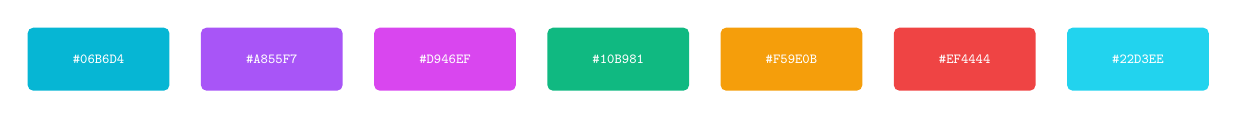
\begin{tikzpicture}
  \foreach \c/\h/\i in {CyberCyan/\#06B6D4/0, NeonPurple/\#A855F7/1, NeonFuchsia/\#D946EF/2, SuccessGreen/\#10B981/3, WarningAmber/\#F59E0B/4, AlertRed/\#EF4444/5, CyberCyanLight/\#22D3EE/6} {
    \fill[\c,rounded corners=2pt] (\i*2.2,0) rectangle (\i*2.2+1.8,0.8);
    \node[text=white,font=\ttfamily\tiny] at (\i*2.2+0.9,0.4) {\h};
  }
\end{tikzpicture}
\end{specbox}

% ===========================================================
\newpage
\section{动效与交互规范}

\subsection{动效原则}

\visid{B-08} 所有动效遵循"有目的、有克制、有反馈"的设计原则。

\begin{center}
\renewcommand{\arraystretch}{1.6}
\begin{tabularx}{\textwidth}{>{\centering\arraybackslash\heiti}p{3cm} >{\centering\arraybackslash}p{3cm} X}
\toprule
\textbf{动效类型} & \textbf{时长/缓动} & \textbf{触发场景} \\
\midrule
Hover 发光 & 300ms / ease & 鼠标悬停卡片，边框亮度增加 \\
页面进入 & 400ms / ease-out & 卡片错落上浮 staggered fade-in-up \\
数据更新 & 600ms / ease-in-out & 数字滚动计数器 Counter Up \\
地图飞行 & 1500ms / cubic-bezier & 城市间跳跃平滑过渡 \\
脉冲标记 & 1500ms / infinite & 地图事件点 animate-ping \\
扫描线 & 持续 / linear & 面板扫描线纹理 15\% 透明度 \\
\bottomrule
\end{tabularx}
\end{center}

\subsection{CSS 变量系统}

\visid{B-09} 系统通过 CSS 自定义属性实现主题统一管理。

\begin{center}
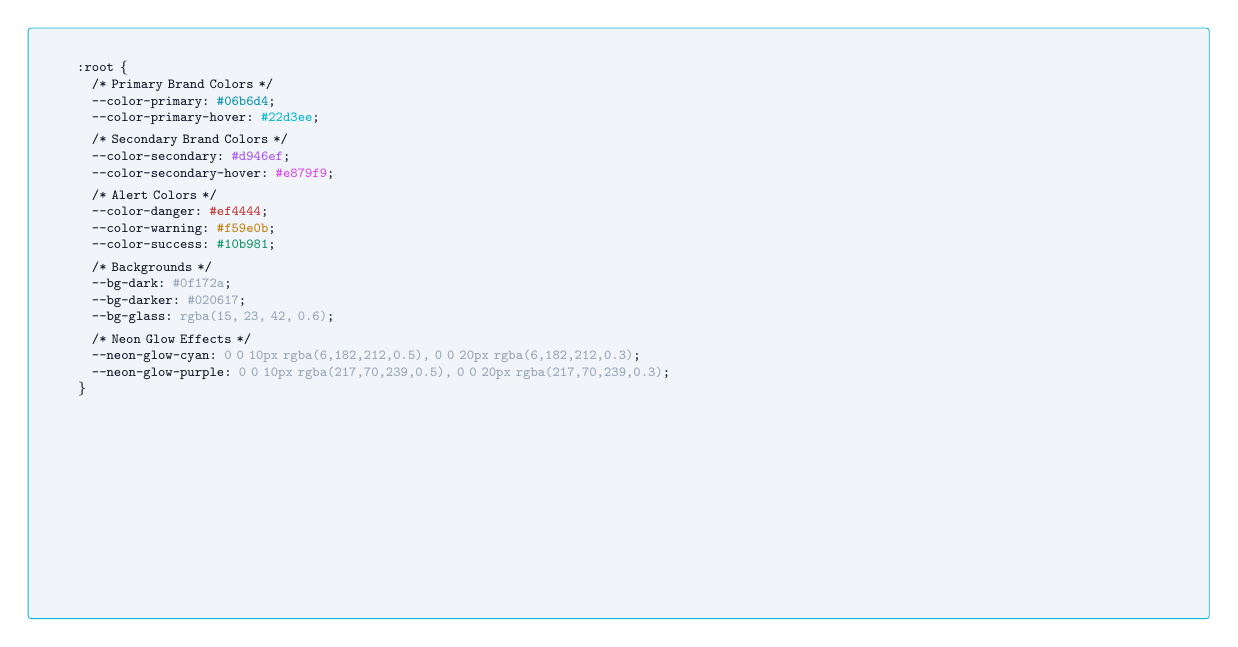
\begin{tikzpicture}
  \fill[LightGray,rounded corners=1pt] (0,0) rectangle (15,7.5);
  \draw[CyberCyan,rounded corners=1pt,line width=0.3pt] (0,0) rectangle (15,7.5);
  \node[anchor=north west,text=DeepBlue,font=\ttfamily\tiny,text width=14cm] at (0.5,7.2) {%
    :root \{\\
    \quad /* Primary Brand Colors */\\
    \quad --color-primary: \textcolor{CyberCyanDark}{\#06b6d4};\\
    \quad --color-primary-hover: \textcolor{CyberCyan}{\#22d3ee};\\[2pt]
    \quad /* Secondary Brand Colors */\\
    \quad --color-secondary: \textcolor{NeonPurple}{\#d946ef};\\
    \quad --color-secondary-hover: \textcolor{NeonFuchsia}{\#e879f9};\\[2pt]
    \quad /* Alert Colors */\\
    \quad --color-danger: \textcolor{AlertRed!80!black}{\#ef4444};\\
    \quad --color-warning: \textcolor{WarningAmber!80!black}{\#f59e0b};\\
    \quad --color-success: \textcolor{SuccessGreen!80!black}{\#10b981};\\[2pt]
    \quad /* Backgrounds */\\
    \quad --bg-dark: \textcolor{TextSecondary}{\#0f172a};\\
    \quad --bg-darker: \textcolor{TextSecondary}{\#020617};\\
    \quad --bg-glass: \textcolor{TextSecondary}{rgba(15, 23, 42, 0.6)};\\[2pt]
    \quad /* Neon Glow Effects */\\
    \quad --neon-glow-cyan: \textcolor{TextSecondary}{0 0 10px rgba(6,182,212,0.5), 0 0 20px rgba(6,182,212,0.3)};\\
    \quad --neon-glow-purple: \textcolor{TextSecondary}{0 0 10px rgba(217,70,239,0.5), 0 0 20px rgba(217,70,239,0.3)};\\
    \}
  };
\end{tikzpicture}
\end{center}

\subsection{Tailwind 扩展配置}

\visid{B-10} 项目 Tailwind CSS 扩展配置与品牌色彩/字体保持同步。

\begin{center}
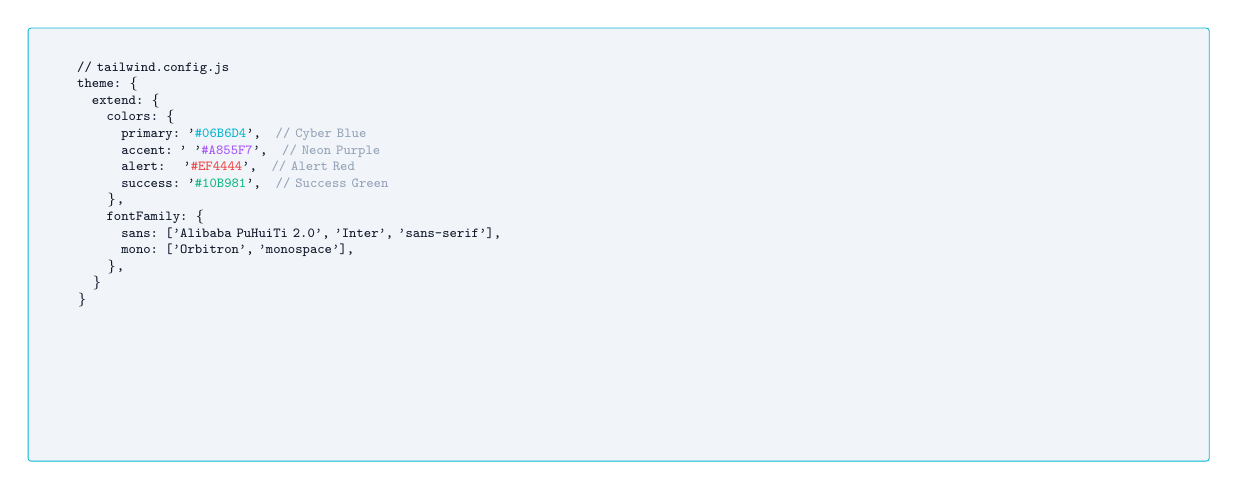
\begin{tikzpicture}
  \fill[LightGray,rounded corners=1pt] (0,0) rectangle (15,5.5);
  \draw[CyberCyan,rounded corners=1pt,line width=0.3pt] (0,0) rectangle (15,5.5);
  \node[anchor=north west,text=DeepBlue,font=\ttfamily\tiny,text width=14cm] at (0.5,5.2) {%
    // tailwind.config.js\\
    theme: \{\\
    \quad extend: \{\\
    \quad\quad colors: \{\\
    \quad\quad\quad primary: '\textcolor{CyberCyan}{\#06B6D4}',\quad\textcolor{TextSecondary}{// Cyber Blue}\\
    \quad\quad\quad accent:\;\,' '\textcolor{NeonPurple}{\#A855F7}',\quad\textcolor{TextSecondary}{// Neon Purple}\\
    \quad\quad\quad alert:\;\;\, '\textcolor{AlertRed}{\#EF4444}',\quad\textcolor{TextSecondary}{// Alert Red}\\
    \quad\quad\quad success: '\textcolor{SuccessGreen}{\#10B981}',\quad\textcolor{TextSecondary}{// Success Green}\\
    \quad\quad \},\\
    \quad\quad fontFamily: \{\\
    \quad\quad\quad sans: ['Alibaba PuHuiTi 2.0', 'Inter', 'sans-serif'],\\
    \quad\quad\quad mono: ['Orbitron', 'monospace'],\\
    \quad\quad \},\\
    \quad \}\\
    \}
  };
\end{tikzpicture}
\end{center}


% C 品牌应用规范
% ==================== C 品牌应用规范 ====================

\newpage
\section{品牌应用规范}

\subsection{名片设计}

\visid{C-01} 名片采用深色主题，正面展示品牌标志与个人信息，背面展示辅助图形。

\begin{center}
\begin{tikzpicture}[scale=0.88]
  % ---- 正面 ----
  \node[font=\heiti\wuhao,text=SlateGray,anchor=south] at (4.25,5.6) {正面};
  \fill[DeepBlue,rounded corners=1pt] (0,0) rectangle (8.5,5.4);
  
  % 左侧青色装饰条
  \fill[CyberCyan] (0,0) rectangle (0.15,5.4);
  
  % Logo
  \node[anchor=north west] at (0.6,4.9) {
\includegraphics[height=1.2cm]{picture/logo.png}};
  
  % 品牌名
  \node[anchor=west,text=white,font=\heiti\sihao] at (0.6,3) {智舆 ZhiYu};
  \node[anchor=west,text=TextSecondary,font=\songti\tiny] at (0.6,2.5) {AI城市舆情态势监测感知与决策推演系统};
  
  % 个人信息
  \draw[CyberCyan,line width=0.3pt,opacity=0.4] (0.6,2) -- (7.9,2);
  \node[anchor=west,text=CyberCyanLight,font=\heiti\scriptsize] at (0.6,1.5) {张\quad 三};
  \node[anchor=west,text=TextSecondary,font=\songti\tiny] at (0.6,1.0) {产品总监 / Product Director};
  \node[anchor=west,text=TextSecondary,font=\ttfamily\tiny] at (0.6,0.5) {zhangsan@zhiyu.ai | +86 138-0000-0000};
  
  % 右下角六边形装饰
  \node[regular polygon,regular polygon sides=6,minimum size=1.2cm,
        draw=CyberCyan,opacity=0.1,line width=0.5pt,rotate=30] at (7.2,1.2) {};
  
  % ---- 背面 ----
  \node[font=\heiti\wuhao,text=SlateGray,anchor=south] at (13.25,5.6) {背面};
  \fill[DeepBlue,rounded corners=1pt] (9,0) rectangle (17.5,5.4);
  
  % 中心大Logo
  \node at (13.25,2.7) {
\includegraphics[height=2.5cm]{picture/logo.png}};
  
  % 六边形网格装饰
  \foreach \x/\y in {10/4.5, 11.2/4.5, 10.6/3.6, 15.2/0.8, 16/1.5, 15.6/0.3} {
    \node[regular polygon,regular polygon sides=6,minimum size=0.6cm,
          draw=CyberCyan,opacity=0.08,line width=0.3pt,rotate=30] at (\x,\y) {};
  }
  
  % 底部网址
  \node[text=TextSecondary,font=\ttfamily\tiny] at (13.25,0.4) {www.zhiyu.ai};
\end{tikzpicture}
\end{center}

\subsection{文档页眉页脚}

\visid{C-02} 正式文档页眉统一展示品牌标志与文档类型，页脚标注版权信息。

\begin{center}
\begin{tikzpicture}
  % 页眉示例
  \fill[white,rounded corners=1pt,draw=MidGray,line width=0.3pt] (0,0) rectangle (15,1.5);
  \node[anchor=west] at (0.3,0.75) {
\includegraphics[height=0.7cm]{picture/logo.png}};
  \node[anchor=west,text=DeepBlue,font=\heiti\scriptsize] at (2.2,0.95) {智舆};
  \node[anchor=west,text=TextSecondary,font=\songti\tiny] at (2.2,0.5) {Visual Identity System};
  \draw[CyberCyan,line width=1pt] (0,0) -- (15,0);
  
  % 页脚示例
  \fill[white,rounded corners=1pt,draw=MidGray,line width=0.3pt] (0,-2) rectangle (15,-0.8);
  \draw[CyberCyan,line width=0.5pt] (0,-0.8) -- (15,-0.8);
  \node[text=TextSecondary,font=\songti\tiny] at (4,-1.4) {\textcopyright\ 2025 智舆 ZhiYu | Confidential};
  \node[text=SlateGray,font=\ttfamily\tiny] at (13,-1.4) {Page 01};
\end{tikzpicture}
\end{center}

\subsection{PPT演示模板}

\visid{C-03} 演示文稿遵循深色主题，16:9比例，标题页与内容页分别定义。

\begin{center}
\begin{tikzpicture}[scale=0.44]
  % ---- 标题页 ----
  \node[font=\heiti\wuhao,text=SlateGray,anchor=south] at (8,9.5) {标题页};
  \fill[DeepBlue,rounded corners=1pt] (0,0) rectangle (16,9);
  
  % 网格背景
  \foreach \x in {0,0.8,...,16} {
    \draw[white,opacity=0.02,line width=0.2pt] (\x,0) -- (\x,9);
  }
  \foreach \y in {0,0.8,...,9} {
    \draw[white,opacity=0.02,line width=0.2pt] (0,\y) -- (16,\y);
  }
  
  % 顶部渐变
  \shade[top color=CyberCyan!15,bottom color=DeepBlue,opacity=0.5] (0,6) rectangle (16,9);
  
  % Logo
  \node at (2.5,7.5) {
\includegraphics[height=1.2cm]{picture/logo.png}};
  
  % 标题
  \node[text=white,font=\heiti\fontsize{18pt}{22pt}\selectfont,anchor=west] at (1,4.5) {演示标题在此};
  \node[text=TextSecondary,font=\songti\scriptsize,anchor=west] at (1,3.5) {副标题 / Subtitle};
  
  % 底部信息
  \draw[CyberCyan,line width=0.5pt,opacity=0.4] (1,1.5) -- (15,1.5);
  \node[text=TextSecondary,font=\songti\tiny,anchor=west] at (1,0.8) {2025 | 智舆团队};
  
  % 右下角装饰
  \node[regular polygon,regular polygon sides=6,minimum size=2cm,
        draw=CyberCyan,opacity=0.08,line width=0.5pt,rotate=30] at (14,2) {};

  % ---- 内容页 ----
  \begin{scope}[shift={(18,0)}]
  \node[font=\heiti\wuhao,text=SlateGray,anchor=south] at (8,9.5) {内容页};
  \fill[DeepBlue,rounded corners=1pt] (0,0) rectangle (16,9);
  
  % 网格
  \foreach \x in {0,0.8,...,16} {
    \draw[white,opacity=0.02,line width=0.2pt] (\x,0) -- (\x,9);
  }
  
  % 顶部栏
  \fill[SlateGray,opacity=0.3] (0,7.8) rectangle (16,9);
  \node[text=CyberCyanLight,font=\heiti\scriptsize,anchor=west] at (0.5,8.4) {章节标题};
  \draw[CyberCyan,line width=1pt] (0,7.8) -- (16,7.8);
  
  % 内容区域
  \fill[SlateGray,opacity=0.2,rounded corners=1pt] (0.8,1) rectangle (7.2,7.4);
  \node[text=TextSecondary,font=\songti\tiny] at (4,4.2) {内容区域 A};
  
  \fill[SlateGray,opacity=0.2,rounded corners=1pt] (7.6,1) rectangle (15.2,7.4);
  \node[text=TextSecondary,font=\songti\tiny] at (11.4,4.2) {内容区域 B};
  
  % 页码
  \node[text=TextSecondary,font=\ttfamily\tiny] at (15,0.4) {02};
  \end{scope}
\end{tikzpicture}
\end{center}

\subsection{系统界面截图规范}

\visid{C-04} 系统截图用于对外宣传时，须遵循以下规范。

\begin{specbox}[截图输出规范]
\begin{itemize}[leftmargin=1.5em,itemsep=2pt]
  \item \textbf{分辨率}：最低 1920$\times$1080 (Full HD)，推荐 2560$\times$1440 (2K)
  \item \textbf{格式}：PNG 无损格式（演示用途），WebP 压缩格式（网页用途）
  \item \textbf{圆角}：外部展示截图添加 16px 圆角 + 4px 阴影
  \item \textbf{背景}：截图外围使用 \texttt{\#0F172A}（Deep Blue）填充
  \item \textbf{水印}：右下角添加半透明品牌标志（20\% 透明度）
  \item \textbf{设备框}：可选添加 MacBook / iPad 设备 Mockup 框架
\end{itemize}
\end{specbox}

\subsection{四级区域可视化配色}

\visid{C-05} 地图四级穿透视图中，各层级使用差异化配色以区分信息层次。

\begin{center}
\begin{tikzpicture}
  % 四级色带
  \foreach \level/\elabel/\zoom/\clr/\y/\desc in {
    全国视图/National/Zoom 4--6/CyberCyan/3/{国境线霓虹描边，省份色块填充},
    省份视图/Province/Zoom 6--8/NeonPurple/2/{省界高亮，地市热力渐变},
    地市视图/City/Zoom 8--12/WarningAmber/1/{城区建筑3D高亮，事件脉冲标记},
    县区视图/District/Zoom 12+/SuccessGreen/0/{街道级舆情详情，原文链接标注}} {
    \fill[\clr,opacity=0.8,rounded corners=1pt] (0,\y) rectangle (3.5,\y+0.8);
    \node[text=white,font=\heiti\scriptsize] at (1.75,\y+0.4) {\level};
    \node[text=SlateGray,font=\songti\tiny,anchor=west] at (3.8,\y+0.55) {\elabel};
    \node[text=TextSecondary,font=\ttfamily\tiny,anchor=west] at (3.8,\y+0.2) {\zoom};
    \node[text=SlateGray,font=\songti\tiny,anchor=west,text width=6cm] at (7,\y+0.4) {\desc};
  }
\end{tikzpicture}
\end{center}

\subsection{网络社交媒体系统}

\visid{C-06} 品牌在社交媒体平台上的视觉标识应用规范。

\begin{center}
\begin{tikzpicture}[scale=0.9]
  % 微信公众号头像
  \node[font=\heiti\wuhao,text=SlateGray,anchor=south] at (2,4.5) {公众号头像};
  \fill[DeepBlue,rounded corners=1pt] (0,0) rectangle (4,4);
  \node at (2,2.3) {
\includegraphics[height=2cm]{picture/logo.png}};
  \node[text=CyberCyanLight,font=\ttfamily\tiny] at (2,0.6) {240 $\times$ 240 px};
  \node[text=TextSecondary,font=\tiny] at (2,0.2) {PNG / 深色背景};
  
  % 微博Banner
  \node[font=\heiti\wuhao,text=SlateGray,anchor=south] at (9.5,4.5) {社交平台 Banner};
  \fill[DeepBlue,rounded corners=1pt] (5,1.2) rectangle (14,4);
  \shade[left color=CyberCyan!20,right color=NeonPurple!15,opacity=0.5] (5,1.2) rectangle (14,4);
  \node[anchor=west] at (5.5,2.6) {
\includegraphics[height=1.5cm]{picture/logo.png}};
  \node[anchor=west,text=white,font=\heiti\sihao] at (7.8,3) {智舆 ZhiYu};
  \node[anchor=west,text=TextSecondary,font=\songti\tiny] at (7.8,2.2) {AI城市舆情态势监测感知与决策推演系统};
  \draw[CyberCyan,line width=0.3pt,opacity=0.4] (7.5,1.8) -- (13.5,1.8);
  \node[text=TextSecondary,font=\ttfamily\tiny] at (9.5,0.6) {1500 $\times$ 500 px};
  \node[text=TextSecondary,font=\tiny] at (9.5,0.2) {JPG / 72dpi};
\end{tikzpicture}
\end{center}

\begin{center}
\begin{tikzpicture}[scale=0.9]
  % 二维码样式
  \node[font=\heiti\wuhao,text=SlateGray,anchor=south] at (2,4.5) {品牌二维码};
  \fill[white,rounded corners=1pt,draw=MidGray,line width=0.3pt] (0,0) rectangle (4,4);
  \fill[DeepBlue,rounded corners=1pt] (0.8,0.8) rectangle (3.2,3.2);
  \node[text=white,font=\ttfamily\tiny] at (2,2.2) {QR Code};
  \node[text=white,font=\tiny] at (2,1.6) {中心嵌Logo};
  \node at (2,2.8) {
\includegraphics[height=0.6cm]{picture/logo.png}};
  \node[text=SlateGray,font=\tiny] at (2,0.4) {前景: Deep Blue / 背景: White};

  % 微信文章页脚
  \node[font=\heiti\wuhao,text=SlateGray,anchor=south] at (9.5,4.5) {文章页脚图};
  \fill[LightGray,rounded corners=1pt] (5,0.5) rectangle (14,4);
  \draw[CyberCyan,line width=0.5pt] (5.5,2.8) -- (13.5,2.8);
  \node[anchor=west] at (5.5,2) {
\includegraphics[height=0.8cm]{picture/logo.png}};
  \node[anchor=west,text=DeepBlue,font=\heiti\scriptsize] at (7.2,2.2) {智舆 ZhiYu};
  \node[anchor=west,text=SlateGray,font=\songti\tiny] at (7.2,1.6) {关注我们，获取最新舆情洞察};
  \node[text=CyberCyanDark,font=\ttfamily\tiny] at (12,1.2) {扫码关注};
  \fill[DeepBlue,rounded corners=1pt] (11.2,1.6) rectangle (12.8,3.2);
  \node[text=white,font=\tiny] at (12,2.4) {QR};
  \node[text=TextSecondary,font=\ttfamily\tiny] at (9.5,0.15) {900 $\times$ 500 px / PNG};
\end{tikzpicture}
\end{center}

\begin{specbox}[社交媒体视觉规范]
\begin{itemize}[leftmargin=1.5em,itemsep=2pt]
  \item 头像统一使用\textbf{深色背景 + 标准Logo}，禁止裁剪或变形
  \item Banner 背景使用品牌渐变（Cyan $\to$ Purple），左侧放置Logo，右侧留白
  \item 二维码前景色固定为 \textbf{Deep Blue}，中心嵌入品牌Logo，尺寸不小于二维码面积的 15\%
  \item 文章页脚图统一版式，底部包含公众号二维码与关注引导语
  \item 所有社交头像须在圆形裁剪后仍保证Logo完整可辨
\end{itemize}
\end{specbox}

% ===========================================================
\newpage
\section{品牌资产清单}

\visid{C-07} 以下为智舆品牌完整资产清单，所有文件按规范命名并归档管理。

\begin{center}
\renewcommand{\arraystretch}{1.5}
\begin{tabularx}{\textwidth}{>{\centering\arraybackslash}p{1cm} >{\heiti}p{3.5cm} p{3cm} X}
\toprule
\textbf{编号} & \textbf{资产名称} & \textbf{格式} & \textbf{用途说明} \\
\midrule
\multicolumn{4}{l}{\textbf{\color{CyberCyan}A 标志文件}} \\
A-01 & Logo 标准版 & PNG / SVG & 深色背景标准使用 \\
A-02 & Logo 反白版 & PNG / SVG & 浅色背景使用 \\
A-03 & Logo 单色版 & PNG / SVG & 印刷受限场景 \\
A-04 & Favicon & ICO / PNG 48px & 浏览器标签图标 \\
\midrule
\multicolumn{4}{l}{\textbf{\color{CyberCyan}B 色彩文件}} \\
B-01 & 品牌色板 & ASE / JSON & 设计软件导入 \\
B-02 & Tailwind 配置 & JS & 前端开发直接引用 \\
B-03 & CSS 变量表 & CSS & 全局主题变量 \\
\midrule
\multicolumn{4}{l}{\textbf{\color{CyberCyan}C 字体文件}} \\
C-01 & Alibaba PuHuiTi 2.0 & TTF / WOFF2 & 中文正文 \\
C-02 & Inter & TTF / WOFF2 & 英文正文 \\
C-03 & Orbitron & TTF / WOFF2 & 科技标题/数字 \\
C-04 & JetBrains Mono & TTF / WOFF2 & 代码/数据 \\
\midrule
\multicolumn{4}{l}{\textbf{\color{CyberCyan}D 模板文件}} \\
D-01 & PPT 演示模板 & PPTX & 对外演示汇报 \\
D-02 & 文档模板 & LaTeX / DOCX & 项目文档撰写 \\
D-03 & 名片模板 & AI / PDF & 印刷输出 \\
\bottomrule
\end{tabularx}
\end{center}

\vspace{12pt}

\begin{center}
\begin{tcolorbox}[
  enhanced,
  colback=CyberCyan!5,
  colframe=CyberCyan,
  boxrule=1pt,
  arc=1pt,
  width=0.85\textwidth,
  halign=center
]
{\heiti\sihao\color{CyberCyanDark} 智舆 ZhiYu}\\[4pt]
{\songti\wuhao\color{SlateGray} AI城市舆情态势监测感知与决策推演系统}\\[8pt]
{\songti\wuhao\color{SlateGray} Visual Identity System v1.0}\\[2pt]
{\songti\wuhao\color{SlateGray} 2025}\\[8pt]
\textcolor{MidGray}{\rule{6cm}{0.3pt}}\\[4pt]
{\songti\tiny\color{TextSecondary} 本手册内容为智舆品牌机密资料，未经授权不得外传复制。}\\
{\songti\tiny\color{TextSecondary} 如需使用品牌素材，请联系品牌管理团队获取授权。}
\end{tcolorbox}
\end{center}


\end{document}
